\documentclass[11pt,letterpaper]{article}
\usepackage[margin=0.95in]{geometry}
\usepackage{amsmath,amssymb,booktabs,graphicx}
\usepackage[hidelinks]{hyperref}
\setlength{\parindent}{0pt}
\setlength{\parskip}{6pt}
\newcommand{\rmse}{\mathrm{RMSE}}
\newcommand{\GGN}{Gauss--Newton}
\newcommand{\loss}{\mathrm{dB}^2}
\title{\textbf{Robust Multi-Position Parametric Room Equalization}\\[4pt]
  \large A Generalized Gauss--Newton Study on Measured Room Responses}
\author{CSE 5403 \enspace $\cdot$ \enspace Algorithms for Nonlinear Optimization}
\date{November 25, 2026}

\begin{document}
\maketitle

\begin{abstract}
We fit a single six-biquad equalizer over 50--500 Hz to measured responses from
multiple microphone positions using a smooth mixture of mean and worst-seat
loss. The implementation uses an analytical response Jacobian and a projected,
damped generalized Gauss--Newton method. On five matched starts, the method
reached the shared stationarity tolerance in a median of 129 objective and
gradient evaluations for the robust objective. L-BFGS-B took 353 and reached
the lowest observed objective. In a spatial holdout of 126 positions, robust
EQ improved worst-seat RMSE over mean EQ in seven of nine training comparisons
and two of nine holdout comparisons. A training-only pilot selected a
$32\rightarrow8\rightarrow2~\loss$ temperature schedule. With identical
starting points and evaluation caps, continuation improved the final objective
once in five comparisons and used more evaluations on all five starts.
Peak-informed placement improved the initial objective against the median
random-center start on every spatial split, and the final objective on four
of nine splits.
\end{abstract}

\section{Problem and research questions}
Moving the listener changes the mix of direct sound and reflected paths.
A peak or cancellation at one listening position can therefore differ from the
response elsewhere. Room equalization surveys describe multi-position
correction as a way to account for that variation during design \cite{cecchi}.
Prior work on low-order parametric IIR design derives analytical derivatives
and discusses multi-point extensions \cite{vairetti}.

We study three questions. How much does a smooth worst-seat term change
training and spatial holdout error? How does a solver that uses the structure
of this term compare with a general-purpose bound-constrained solver? Does a
gradual reduction of the temperature find a better endpoint at the same final
temperature? The course contribution is the derivation, implementation, and
controlled measurement of those choices on the same equalization problem.

\clearpage
\section{Signal model and preprocessing}
Let $h_{mj}$ be the measured log magnitude in dB at receiver $m$ and
frequency $f_j$. Each measurement is a 32,768-sample room impulse response
at 48 kHz. We use a full-length rectangular window, a 32,768-point real FFT, a
magnitude floor of $10^{-12}$ before the logarithm, and linear interpolation
in Hz on the resulting dB spectrum. There is no spectral smoothing.
The evaluation grid comprises 128 logarithmically spaced frequencies between
50 and 500 Hz, each with weight $w_j=1/128$.

The equalizer is a cascade of $K=6$ peaking biquads with parameters
$\theta_k=(g_k,\log f_k,\log Q_k)$. The bounds are
$-12\leq g_k\leq6$ dB, $50\leq f_k\leq500$ Hz, and $0.3\leq Q_k\leq10$.
The cascade response $u_j(\theta)$ is the sum of the individual dB
responses. A flat target is defined by a common level $T$ estimated from
training data. Every receiver in a split uses that same $T$. The predicted
corrected dB magnitude is $h_{mj}+u_j$.

\subsection{Analytical response derivative}
For one biquad, let $\omega_0=2\pi f_k/f_s$, $A=10^{g_k/40}$,
$a=\sin\omega_0/(2Q_k)$, and $c=\cos\omega-\cos\omega_0$.
The cookbook coefficients \cite{rbj}, after factoring the common
$2e^{-i\omega}$ term out of each response polynomial, give
\[
  H(e^{i\omega})=\frac{c+i a A\sin\omega}{c+i(a/A)\sin\omega}.
\]
For $N=c+i a A\sin\omega$ and $D=c+i(a/A)\sin\omega$,
\[
  \partial_\xi\,20\log_{10}|H|
    =\frac{20}{\log 10}\Re\!\left(\frac{\partial_\xi N}{N}
                         -\frac{\partial_\xi D}{D}\right).
\]
Writing $c=-2\sin((\omega+\omega_0)/2)\sin((\omega-\omega_0)/2)$
avoids subtracting nearby cosines. The chain rule uses
$\partial_g A=(\log 10) A/40$,
$\partial_{\log Q}a=-a$,
$\partial_{\log f}c=\omega_0\sin\omega_0$, and
$\partial_{\log f}a=\omega_0\cos\omega_0/(2Q)$.
At zero gain, the two polynomials coincide and the frequency and $Q$
derivatives vanish. The near-flat start therefore uses nonzero gains.

The optimizer constrains each biquad independently. We estimate the
maximum combined boost on 8,192 log-spaced frequencies from 1 Hz to
Nyquist. This diagnostic measures the headroom demand of overlapping
filters. It can exceed the per-filter $+6$ dB bound.

\clearpage
\section{Loss, curvature, and an analytical benchmark}
The weighted residual and loss for seat $m$ are
\[
 r_{mj}=\sqrt{w_j}(h_{mj}+u_j-T),\qquad
 e_m=\tfrac12\|r_m\|_2^2.
\]
With $M$ training seats, $R(\theta)=\tfrac12\sum_k g_k^2$, and
$\lambda=0.01$, the optimized objective is
\[
 F_{\alpha,\tau}(\theta)
 =\alpha\,\overline e+
 (1-\alpha)\tau\log\!\left(\frac1M\sum_{m=1}^M e^{e_m/\tau}\right)
 +\lambda R(\theta).
\]
At $\alpha=1$ this is the regularized mean loss. As $\tau$ decreases, the
smooth term approaches the maximum seat loss. Indeed, for
$E=\max_m e_m$, the term lies between $E-\tau\log M$ and $E$.
The implementation shifts losses by $E$ before exponentiation and uses
a separate evaluation for near-zero scaled differences to retain accuracy
at large temperatures. Pooled RMSE is $\sqrt{2\overline e}$.
Worst-seat RMSE is $\max_m\sqrt{2e_m}$.

\subsection{Generalized Gauss--Newton matrix}
Let $J=\partial r_m/\partial\theta$ be the common weighted Jacobian.
Define the seat gradient $a_m=J^\top r_m$ and the probability
$p_m=\exp(e_m/\tau)/\sum_\ell\exp(e_\ell/\tau)$.
For $q_m=\alpha/M+(1-\alpha)p_m$, differentiation gives
\[
 g=\sum_m q_m a_m+\lambda\nabla R,\qquad
 B=J^\top J+\frac{1-\alpha}{\tau}
      \sum_m p_m (a_m-\bar a_p)(a_m-\bar a_p)^\top+\lambda\nabla^2R ,
\]
where $\bar a_p=\sum_m p_m a_m$. In the generalized Gauss--Newton
approximation, the Hessian contributions from second derivatives of $r_m$
are dropped and the outer-loss curvature is retained \cite{schraudolph}.
The covariance expression and the diagonal gain regularizer are positive
semidefinite. Centering the seat gradients before forming their covariance
avoids a subtraction of matrices with large entries.

\subsection{Unrestricted mean-error floor}
For any $j$, the mean squared corrected error decomposes as
\[
  \frac1M\sum_m(h_{mj}+u_j-T)^2
   =\operatorname{Var}_m(h_{mj})+(\overline h_j+u_j-T)^2.
\]
Consequently the unrestricted mean squared error is at least
$\sum_j w_j\operatorname{Var}_m(h_{mj})$, attained at
$u_j=T-\overline h_j$. Its square root is a pooled RMSE floor.
This comparison drops the filter parameterization and gain penalty.
It addresses the unregularized mean error on a fixed set of seats.
The same decomposition shows that shared EQ preserves the pointwise
spread across seats while changing their errors relative to the target.

\clearpage
\section{Bound-constrained optimization}
\subsection{Projected damped generalized Gauss--Newton}
Let $\mathcal B$ denote the box of allowed parameters and $\Pi_{\mathcal B}$
be componentwise clipping. At a feasible iterate $x$, the solver measures
stationarity by $\|x-\Pi_{\mathcal B}(x-g)\|_\infty$.
It fixes variables at an active bound when the negative gradient points
outside the box. For the remaining indices, it solves the free block of
$(B+\mu D)d=-g$, with $D_{ii}=\max(B_{ii},10^{-3})$.
The initial damping is $\mu=10^{-3}$. A direct linear solve uses the small
free block of the 18-parameter system.

At backtracking attempt $j$, let
$s_j=\Pi_{\mathcal B}(x+2^{-j}d)-x$. The solver evaluates candidates only if
$g^\top s_j<0$. It requires a strict decrease and the projected Armijo
condition $F(x+s_j)\leq F(x)+10^{-4}g^\top s_j$.
If backtracking along the damped direction fails, the solver tries the
diagonally scaled negative gradient $-D^{-1}g$ with the same test. Damping is
reduced after a full Gauss--Newton step and increased after a shortened step
or a gradient fallback. The trace records accepted objectives, projected
gradient norms, damping, and evaluation counts.

\subsection{Reference solver and stopping rules}
L-BFGS-B uses the same analytic objective and gradient and the same box
constraints \cite{byrd}. The two solvers share the same five start vectors,
a $10^{-4}$ projected-gradient tolerance, and an evaluation cap of 2,500.
L-BFGS-B also has a relative objective tolerance of $10^{-13}$.
The reported stationarity flag is based on the common projected norm.
Each joint objective and gradient call counts once. The custom solver also
forms the generalized curvature at every scored candidate and logs that
count separately. An evaluation comparison measures calls and a runtime
comparison measures the overall implementation on the available machine.

The near-flat start places six centers geometrically inside the band at
$-1$ dB and $Q=1$. Other starts add seeded Gaussian perturbations in the
parameter coordinates and clip to the box. The common seeds are 11, 23, 37,
and 59. Optimization remains nonconvex under this parameterization. Different
stationary points are expected, and the best observed value is an empirical
reference.

\subsection{Numerical checks}
Tests compare the cascade with an independent SciPy SOS evaluation, check
stability and the unity response at zero gain, and compare the analytical
gradient and Jacobian with central finite differences. They verify symmetric
positive semidefinite curvature, the limiting behavior of the temperature,
variance invariance, and the mean-error floor. Bounds and decreasing
accepted objectives are checked on a constrained quadratic and checked
again on the recorded room-EQ fits.

\clearpage
\section{Data and experimental design}
MeshRIR is a public dataset of densely measured room responses \cite{mesh}.
We used the single-source S1-M3969 NumPy archive in release 1.2
\cite{release}. Its checksum is recorded in the run manifest. The archive
contains 3,969 positions on a $21\times21\times9$ grid with 5 cm spacing.
The benchmark uses the middle horizontal plane at $z=0$ and the single
source at $(2.0,1.5,0.0)$ m in the dataset coordinate system.

\subsection{Matched solver benchmark}
A deterministic random split of the middle plane supplies nine training
seats and twelve held-out seats. The grand mean training dB magnitude
defines the shared target. The benchmark compares the solvers on mean
loss and on robust loss with $\alpha=0.5$ and $\tau=2~\loss$.
For each solver and loss, the lowest training-objective fit among five
starts is used for the acoustic metrics. The twelve-position split checks
nearby unmeasured positions and has no spatial exclusion buffer.

\subsection{Spatial holdout}
The right-hand strip at $x\geq0.25$ m supplies 126 fixed test positions.
Training positions are drawn from $x\leq0$ m, leaving a horizontal gap of
at least 25 cm. Each of three seeds supplies nested training sets of 3,
10, and 20 positions. The center receiver, index 1984, is included in
every training set. It defines the shared level reference and supplies the
single-seat training response. The common anchor keeps the target
comparable across different training counts.

The spatial comparisons use no EQ, single-seat EQ, mean EQ, and the
smooth robust objective with $\alpha\in\{0,0.25,0.5,0.75,1\}$ at
$\tau=2~\loss$. The $\alpha=1$ endpoint is the mean fit. Each
optimized condition uses three identical L-BFGS-B starts and selects the
fit by its training objective. Held-out data are used for scoring.
The primary robustness comparison uses $\alpha=0.5$. We report the
paired difference between robust and mean errors for each training seed
and count, interpreting the three nested repeats descriptively.

\subsection{Temperature ablation}
Continuation uses the same custom solver as the direct condition.
The pilot compares three geometric schedules ending at $2~\loss$ on
three six-seat subsets of the nine designated training seats. Each
subset excludes a different third of the training set. Two separate
initializations per subset give six comparisons per schedule. We rank
schedules by median paired improvement in the final-temperature training
objective, with median evaluation use as a tie-breaker.
The selected schedule is then compared with direct fitting on all nine
training seats from the five benchmark starts.

\clearpage
\section{Matched solver results}
\begin{table}[h!]
\centering
\small
\begin{tabular}{llrrrrr}
\toprule
Loss & Solver & Stationary & Median $F$ & Best $F$ & Median calls & Median ms \\
\midrule
Mean & Gauss--Newton & 5/5 & 11.389 & 10.212 & 116 & 11 \\
Mean & L-BFGS-B      & 5/5 & 10.350 & 10.125 & 399 & 79 \\
Robust & Gauss--Newton & 5/5 & 11.191 & 10.995 & 129 & 20 \\
Robust & L-BFGS-B      & 5/5 & 12.232 & 10.915 & 353 & 87 \\
\bottomrule
\end{tabular}
\caption{Matched outcomes over five starts per solver and loss. Objective
values are in $\loss$. Compare objective values within the same loss.}
\end{table}

\begin{figure}[h!]
\centering
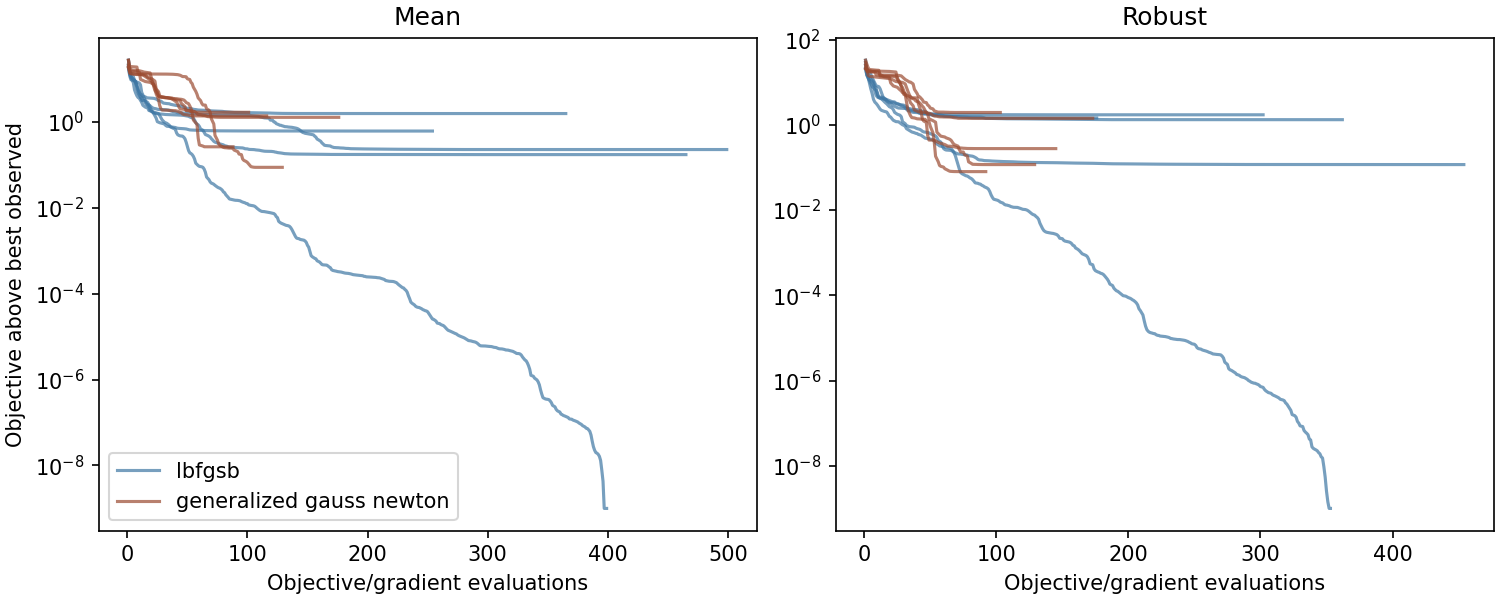
\includegraphics[width=\linewidth]{results/main/convergence.png}
\caption{Accepted iterates against evaluation count. Each panel uses the
best observed value for its loss as the reference.}
\end{figure}

The custom method needed fewer evaluations for both losses in this
benchmark. Its robust-loss median objective was lower, while L-BFGS-B
reached the lowest objective across starts. For mean loss, L-BFGS-B
also had the lower median objective. These differences separate the speed
of reaching stationarity from the quality of the stationary point.

On the nine training seats, the unrestricted pooled RMSE floor was
3.614 dB. The best-training-objective L-BFGS-B mean fit reached
4.289 dB of training pooled RMSE, about 0.676 dB above that floor.
This separation includes the effects of parameterization, gain
regularization, and local optimization. On the twelve-position test split,
L-BFGS-B mean EQ changed pooled and worst-seat RMSE from 6.845 and
8.128 dB to 4.498 and 5.976 dB. Its robust fit reached 4.531 and 5.897 dB.

\clearpage
\section{Spatial generalization}
\begin{table}[h!]
\centering
\small
\begin{tabular}{rlrr}
\toprule
Training seats & Method & Pooled RMSE & Worst-seat RMSE \\
\midrule
Any & No EQ & 7.729 & 9.015 \\
Any & Single-seat EQ & 4.926 & 6.167 \\
3 & Mean EQ & 4.933 & 6.175 \\
3 & Robust EQ & 4.944 & 6.239 \\
10 & Mean EQ & 5.026 & 6.229 \\
10 & Robust EQ & 5.096 & 6.296 \\
20 & Mean EQ & 5.100 & 6.323 \\
20 & Robust EQ & 5.130 & 6.360 \\
\bottomrule
\end{tabular}
\caption{Median spatial holdout RMSE over the three training seeds,
in dB. Robust EQ uses $\alpha=0.5$.}
\end{table}

\begin{figure}[h!]
\centering
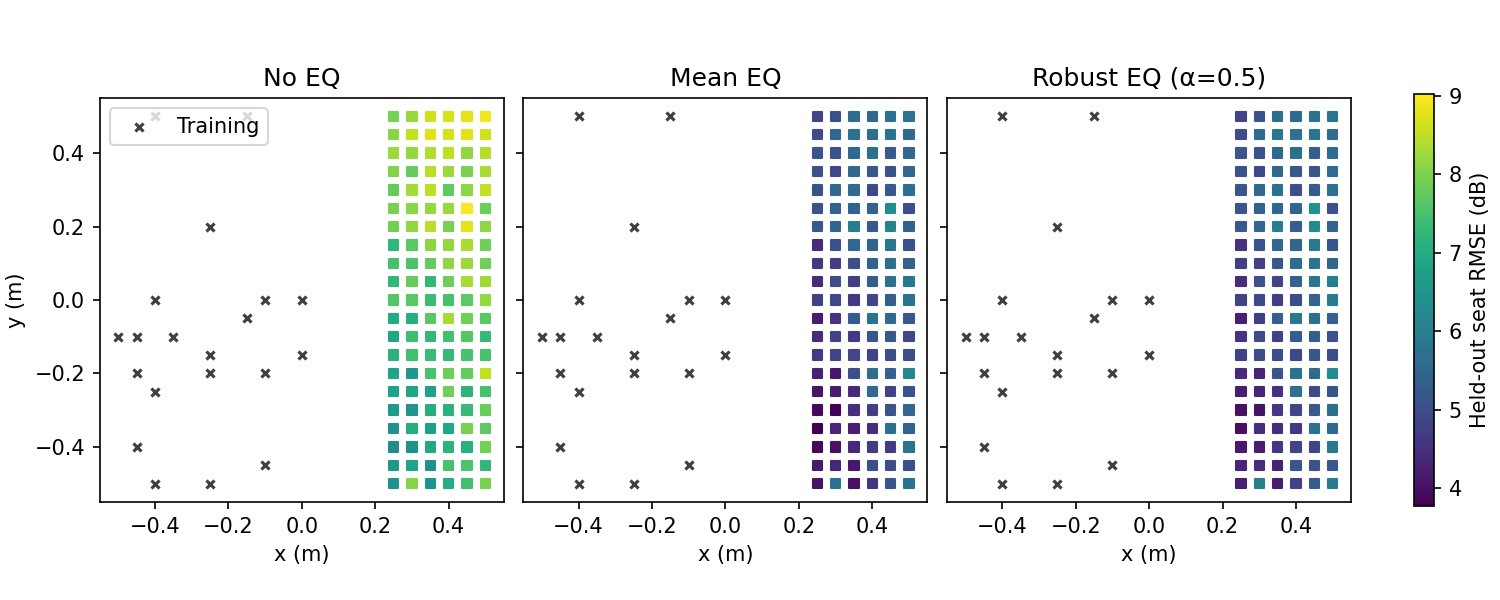
\includegraphics[width=0.98\linewidth]{results/main/spatial_map.png}
\caption{Seat RMSE on the fixed holdout for seed 101 and twenty training
positions. The cross markers identify the training positions. All panels
use the same color scale.}
\end{figure}

Both multi-seat designs reduced the holdout error relative to no EQ, and
the anchor-only fit was competitive on this block. With $\alpha=0.5$,
robust EQ lowered worst-seat error in seven of nine training comparisons.
The paired median difference was $-0.036$ dB, with an interquartile
interval of $[-0.137,-0.030]$ dB. On the holdout, it lowered worst-seat
error in two of nine comparisons. The median difference was $+0.064$ dB,
with interquartile interval $[+0.014,+0.090]$ dB. For pooled RMSE, the
median paired differences were $+0.038$ dB in training and $+0.035$ dB
on the holdout. Thus the primary robust objective tended to improve its
training worst seat at the expense of a small pooled error increase.
That worst-seat benefit rarely carried to the reserved block.

\clearpage
\subsection{Paired effects and training count}

\begin{figure}[h!]
\centering
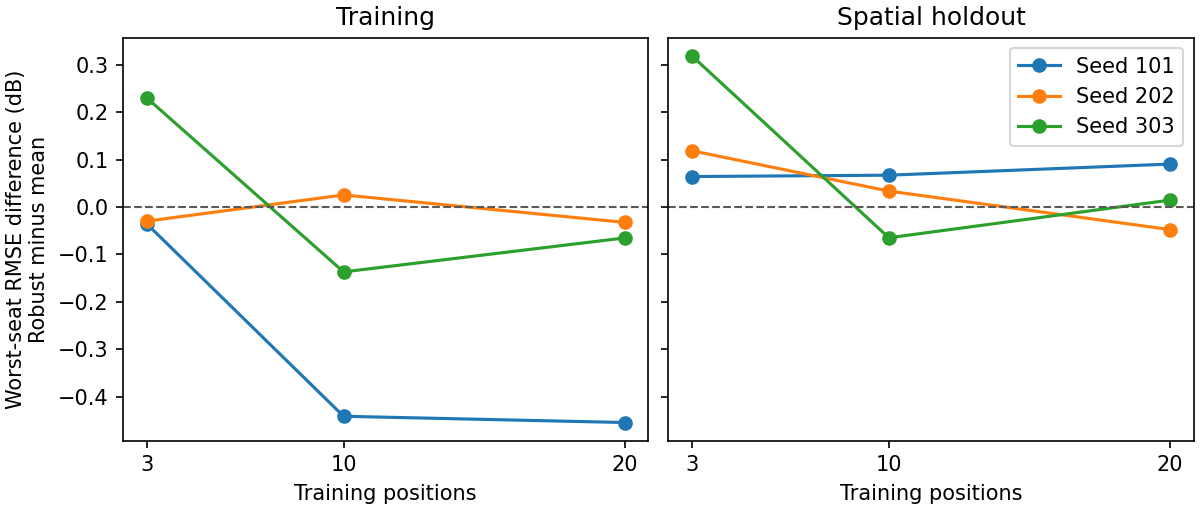
\includegraphics[width=0.92\linewidth]{results/ablation/paired_worst_seat.png}
\caption{Paired worst-seat RMSE differences for robust minus mean EQ.
Negative values favor robust EQ. Lines connect nested training counts
within the same seed.}
\end{figure}

The median paired worst-seat difference favored robust EQ in training
at every count, and favored mean EQ on the holdout at every count.
In this geometry, adding training seats improved coverage of the
training region while leaving the test strip outside that region.
The median holdout error did not improve as the number of training seats
increased for either of the two primary multi-seat fits.

\begin{figure}[h!]
\centering
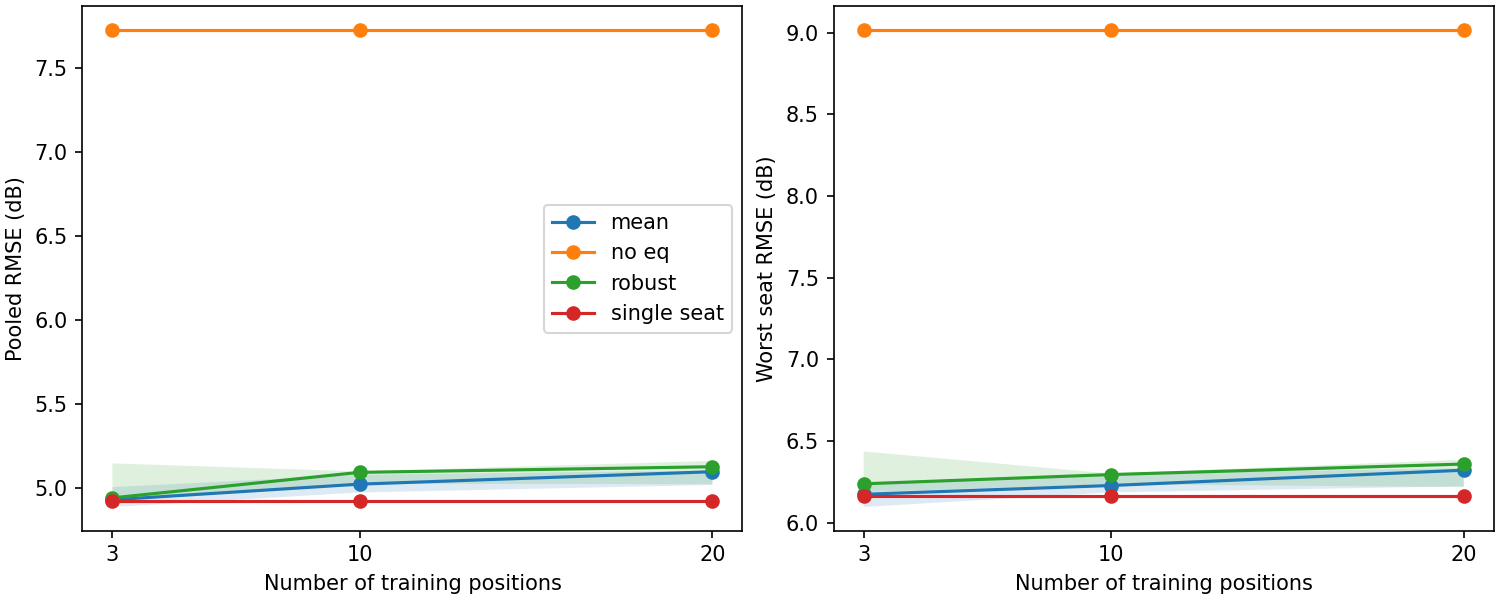
\includegraphics[width=\linewidth]{results/main/spatial_holdout.png}
\caption{Held-out error by training count. Lines give the median of three
training selections and shaded regions give their interquartile ranges.
The no-EQ and single-seat responses are shared across training selections.}
\end{figure}

\clearpage
\section{Temperature continuation}
The candidates were $8\rightarrow4\rightarrow2$,
$18\rightarrow6\rightarrow2$, and $32\rightarrow8\rightarrow2$,
in $\loss$. Their pilot median paired objective differences relative to
direct fitting were $-0.801$, $+0.463$, and $-0.915$, respectively.
The pilot selected the third schedule.
For the benchmark each early stage could use at most 250 of the 2,500
per-fit calls, and the final stage received all remaining calls. Each
stage starts from the preceding parameters and reinitializes damping.
The direct run places its entire cap at $\tau=2$.

\begin{table}[h!]
\centering
\small
\begin{tabular}{lrrrrr}
\toprule
Start & Direct $F$ & Continuation $F$ & $\Delta F$ & Direct calls & Cont.\ calls \\
\midrule
Near-flat & 11.191 & 12.500 & $+1.309$ & 145 & 496 \\
Seed 11   & 12.856 & 11.433 & $-1.422$ & 103 & 233 \\
Seed 23   & 11.031 & 14.769 & $+3.738$ & 129 & 225 \\
Seed 37   & 10.995 & 11.243 & $+0.249$ & 92  & 218 \\
Seed 59   & 12.330 & 12.500 & $+0.170$ & 173 & 416 \\
\midrule
Median    & 11.191 & 12.500 & $+0.249$ & 129 & 233 \\
\bottomrule
\end{tabular}
\caption{All objectives evaluated at the final temperature
$\tau=2~\loss$. $\Delta F$ is continuation minus direct within a start.
The median of the paired differences is shown in the final row.}
\end{table}

All ten final fits satisfied the $10^{-4}$ projected-gradient threshold.
The median projected norm was $8.8\times10^{-5}$ for the direct
condition and $5.9\times10^{-5}$ for continuation. Continuation improved
one matched objective and used more calls on all five starts.
Its best value, 11.243, exceeded the best direct value, 10.995.
On these data, beginning with more uniform seat weights changed the
stationary point reached, sometimes toward a higher final objective.
The small pilot and five-start benchmark limit claims about alternative
schedules or other filters.

At higher temperatures, the softmax weights become more uniform and
the search follows an objective closer to mean loss. A stationary point
of that early objective can warm-start a different basin at the final
temperature. In this ablation the extra stages cost between 96 and 351
calls relative to direct fitting. A continuation advantage would have to
offset that work with a better endpoint or a more reliable fit.

\clearpage
\section{Peak-informed initialization}
We ranked local positive peaks in the median training response by height.
The initializer accepted peaks at least one-sixth octave apart and placed
one cut at each accepted frequency, up to six. Peak gains were minus half
the peak height, with the cut magnitude limited to 1--5 dB. Each filter used
$Q=1$. All ten benchmark splits supplied six eligible peaks. The
implementation can fill unused sections in gaps at $-1$ dB.

For each split, the comparison used one peak-informed start, five seeded
random-center starts, and the conventional near-flat start. The random
starts drew separated centers on a log-frequency scale and copied the
peak fit's initial gains and $Q$ values in frequency order. This controls
for initial cut strength in the peak-versus-random comparison. The near-flat
reference used geometrically spaced centers and $-1$ dB gains. All fits
used the same generalized Gauss--Newton solver, $\alpha=0.5$, $\tau=2~\loss$,
parameter bounds, 2,500-call cap, and $10^{-4}$ projected-gradient tolerance.

\begin{table}[h!]
\centering
\small
\begin{tabular}{lrrr}
\toprule
Start & Initial $F$ & Final $F$ & Evaluations \\
\midrule
Near-flat & 28.744 & 11.280 & 132 \\
Peak-informed & 79.098 & 10.950 & 126 \\
Random centers & 90.122 & 10.873 & 107 \\
\bottomrule
\end{tabular}
\caption{Median across nine spatial training splits. Each split contributes
one value for the peak and near-flat starts and the median across five random
starts. Objective values are in $\loss$.}
\end{table}

On the nine spatial training splits, the peak start had a lower initial
objective than the median of the matched random-center starts in all nine
comparisons. After optimization it had a lower final objective in four,
with a median paired difference of $+0.639~\loss$. It used fewer evaluations
in one of nine comparisons, tied once, and used a median of 18 extra
evaluations relative to the split-level random median. On the nine-seat
solver benchmark, the peak, near-flat, and median random final objectives
were 11.146, 11.191, and 10.995, respectively. All 70 fits attained the
stationarity tolerance.

The favorable initial comparison at matched cut strength did not establish
a consistent advantage after optimization. The near-flat reference started
from a lower aggregate objective, suggesting that initial cut strength and
overlap matter alongside center placement. The comparisons here isolate
placement against the matched random starts and characterize the tested
choice of cut strength against the near-flat reference.

\clearpage
\section{Limitations and conclusions}
This experiment uses one source, one room, a one-meter-wide plane, and one
fixed spatial holdout. Nearby measurements are correlated, the training
sets are nested, and the held-out positions are reused across comparisons.
The results describe this acoustic region. Generalization across rooms,
source placements, and larger listening areas remains unmeasured.

The objective measures magnitude response in a low-frequency band. There
are no listening judgments or phase or decay-time criteria. The shared
target is flat, and a single common level reference leaves level differences
between seats in the error. Median maximum boost of the primary robust
fit ranged from 7.95 to 10.98 dB across training counts, which is relevant
to playback headroom. The experiment includes box bounds on individual
filters and monitors total boost. The reported error improvements describe
the numerical response model.

Structured curvature reduced calls to stationarity. The lowest objective
depended on the solver and start. Worst-seat improvements were more frequent
on the training seats than on the separated holdout. The tested continuation
schedule typically increased the objective and consistently increased call
counts. Peak placement improved initial objectives at matched cut strength,
with mixed final outcomes.

\subsection*{Reproducibility}
The project uses Python 3.13 and the versions pinned in
\texttt{uv.lock}. From the project root after dataset verification:
\begin{verbatim}
.\.venv\Scripts\python.exe -m room_eq.experiments
.\.venv\Scripts\python.exe -m room_eq.ablation
.\.venv\Scripts\python.exe -m room_eq.peak_ablation
\end{verbatim}
The main manifest records split IDs and the fitted settings.
The ablation manifest records pilot configuration and the chosen schedule.
CSV files give the aggregate and paired results, and JSON Lines files
include per-start parameters and convergence traces.

\begin{thebibliography}{9}
\small
\setlength{\itemsep}{0pt}
\setlength{\parskip}{0pt}
\bibitem{cecchi} S. Cecchi, A. Carini, and S. Spors.
Room Response Equalization---A Review. \emph{Applied Sciences}, 8(1), 16,
2018. \href{https://doi.org/10.3390/app8010016}{doi:10.3390/app8010016}.
\bibitem{vairetti} G. Vairetti et al. An Automatic Design Procedure for
Low-Order IIR Parametric Equalizers. \emph{J. Audio Eng. Soc.},
66(11), 935--952, 2018.
\href{https://doi.org/10.17743/jaes.2018.0049}{doi:10.17743/jaes.2018.0049}.
\bibitem{rbj} R. Bristow-Johnson, adapted by the W3C Audio Working Group.
\emph{Audio EQ Cookbook}, 2021.
\href{https://www.w3.org/TR/audio-eq-cookbook/}{W3C Working Group Note}.
\bibitem{schraudolph} N. N. Schraudolph. Fast Curvature Matrix-Vector
Products for Second-Order Gradient Descent. \emph{Neural Computation},
14(7), 1723--1738, 2002.
\href{https://doi.org/10.1162/08997660260028683}{doi:10.1162/08997660260028683}.
\bibitem{byrd} R. H. Byrd, P. Lu, J. Nocedal, and C. Zhu.
A Limited Memory Algorithm for Bound Constrained Optimization.
\emph{SIAM J. Sci. Comput.}, 16(5), 1190--1208, 1995.
\href{https://doi.org/10.1137/0916069}{doi:10.1137/0916069}.
\bibitem{mesh} S. Koyama et al. MeshRIR: A Dataset of Room Impulse Responses
on Meshed Grid Points for Evaluating Sound Field Analysis and Synthesis
Methods. \emph{IEEE WASPAA}, 2021.
\href{https://arxiv.org/abs/2106.10801}{arXiv:2106.10801}.
\bibitem{release} S. Koyama et al. MeshRIR dataset, version 1.2, 2024.
CC BY 4.0. \href{https://doi.org/10.5281/zenodo.10852693}{doi:10.5281/zenodo.10852693}.
\end{thebibliography}
\end{document}
